%% skycell --- manuscript for Astronomy and Computing (Elsevier), on the journal's
%% template (elsarticle-template-harv.tex, elsarticle v3.3): final 5p two-column
%% layout, author-year citations.
%%
%% Build:  make            -> skycell.pdf
%%         make submission -> submission/, one self-contained .tex with the figure
%%                            and the highlights, ready to upload
%% The text is content.tex; the references are refs.tex.
\documentclass[final,5p,times,twocolumn,authoryear]{elsarticle}

%% graphicx is loaded by elsarticle
\usepackage{amsmath}
\usepackage{amssymb}
\usepackage{url}
\usepackage[bookmarks=false,colorlinks=true,linkcolor=black,citecolor=black,urlcolor=blue]{hyperref}

%% astronomical units, and the word used for section references
\newcommand{\arcsec}{\ensuremath{^{\prime\prime}}}
\newcommand{\arcmin}{\ensuremath{^{\prime}}}
\newcommand{\degr}{\ensuremath{^{\circ}}}
\newcommand{\Sect}{Section}

\journal{Astronomy $\&$ Computing}

\begin{document}

\begin{frontmatter}

\title{skycell: a cost-based HEALPix index for sky positions in PostgreSQL}

\author[skao]{Jes\'us Salgado\corref{cor}}
\ead{jesus.salgado@skao.int}
\author[skao]{Michele Delli Veneri}
\ead{michele.delliveneri@skao.int}
\cortext[cor]{Corresponding author}
\affiliation[skao]{organization={SKA Observatory},
  addressline={Jodrell Bank, Lower Withington},
  city={Macclesfield},
  postcode={SK11 9FT},
  country={United Kingdom}}

\begin{abstract}
Astronomical archives answer positional queries from relational databases, and in
PostgreSQL two extensions dominate: Q3C, which keys sources by a cube quad-tree index in
a B-tree, and pgSphere, which stores spherical geometry in a GiST tree and also indexes
regions. We present \texttt{skycell}, a PostgreSQL extension that keeps the integer key
and the B-tree yet answers cones, polygons, cross-matches and stored footprints in the
archives' own ADQL vocabulary. Positions are keyed by their order-29 HEALPix cell, and a
query region is covered by cells whose depth is chosen by a cost model: the price of an
extra index range against the false-positive rows it removes, with local source density
read from the histogram PostgreSQL already keeps. Cones and cross-matches are answered by
a planner custom scan that walks the covering's ranges, polygons by a rewrite into range
conditions, and stored regions by a GiST operator class. Coverings are validated by
brute force over millions of points. In randomized paired trials on PostgreSQL 18.6 with
10- and 50-million-row catalogues, including real Gaia DR3 positions, \texttt{skycell}
is faster than pgSphere at every cone radius from 1\arcsec\ to 3\degr, by 4--33\% with a
warm cache and up to 2.7 times cold. It cross-matches 20--33\% faster than Q3C's
\texttt{q3c\_join} and three times faster than pgSphere, and answers convex polygons
2.7--4.4 times faster than pgSphere, from an index a third the size. One index serving
points, regions and cross-matches through ADQL makes \texttt{skycell} a strong default
for an archive's positional layer.
\end{abstract}

\begin{highlights}
\item A HEALPix B-tree index for PostgreSQL answering cones, polygons and cross-matches
\item A cost model sets each covering's depth from local density and index range price
\item Faster than pgSphere at every cone radius from 1 arcsec to 3 deg, real Gaia DR3 too
\item Cross-matches 20--33\% faster than q3c\_join, from an index a third of pgSphere's size
\item Speaks ADQL; one column holds circles and polygons, read and written as IVOA STC-S
\end{highlights}

\begin{keyword}
%% up to 6 keywords
Astronomical databases \sep Spatial indexing \sep HEALPix \sep PostgreSQL \sep
Cross-matching \sep Virtual Observatory
\end{keyword}

\end{frontmatter}

%% The paper's text, from the Introduction to the Conclusions, input by skycell.tex,
%% which defines \Sect (the word used for section references).

\section{Introduction}

Most questions asked of an astronomical archive are positional: which sources lie in
this cone, which observations cover this field, which catalogue sources match my target
list. In the Virtual Observatory they arrive as ADQL \citep{adql}
through the Table Access Protocol \citep{tap}, usually generated by a service layer
\citep[e.g.][]{dachs}, and at the scale of the ESA Gaia Archive
\citep{gaiaarchive1, gaiaarchive2}, which serves about $10^9$ sources and offers
server-side cross-matching.

For those who run such archives the questions are practical: how fast cone searches
and cross-matches are on a large catalogue, how large the index is, how long it takes to
build and how much memory it needs, whether performance holds in crowded fields and at
scale, and how much an existing database has to change. In PostgreSQL the usual answers
are two extensions. Q3C
\citep{q3c} stores each position as a 64-bit integer from a quad-tree on a cube in a
B-tree: compact and fast for points, with \texttt{q3c\_join} for cross-matching.
pgSphere \citep{pgsphere} stores spherical geometry in a GiST tree: more general, and
able to index stored regions such as observation footprints. Archives that need both kinds of query often run both. Related designs
include the Hierarchical Triangular Mesh \citep{htm} and the zones algorithm
\citep{zones}.

This paper presents \texttt{skycell}, a PostgreSQL extension that covers both roles
with one index and ADQL's own vocabulary. Positions are stored as an integer HEALPix cell
in an ordinary B-tree, as in Q3C, but how a query region becomes index ranges is chosen
per query by a cost model from statistics PostgreSQL already keeps. Stored regions get
their own GiST index. \Sect~\ref{sec:method} explains how
both indexes work, \Sect~\ref{sec:validation} why they do not miss rows,
\Sect~\ref{sec:adql} how to use them in an existing archive, \Sect~\ref{sec:tests}
how they compare with Q3C and pgSphere, and \Sect~\ref{sec:conclusions} when
\texttt{skycell} is worth adopting.

\section{How skycell works}
\label{sec:method}

\subsection{Positions as integers}
\label{sec:key}

A B-tree can only answer range conditions on a sortable key, so a position on the sky
has to become a number first. \texttt{skycell} uses the position's HEALPix cell at order
29 in the nested scheme \citep{healpix}: a 64-bit integer, with cells about 0.4\,mas
across. Three properties of this key matter. First, cells are \emph{nested}: all the
order-29 cells inside a larger cell $p$ at order $k$ form one contiguous run of
integers,
\begin{equation}
  \bigl[\, p\cdot 4^{\,29-k},\; (p+1)\cdot 4^{\,29-k} - 1 \,\bigr],
  \label{eq:interval}
\end{equation}
so any region covered by cells of any size becomes a set of integer ranges that the
B-tree answers with range scans. Second, cells have \emph{equal area}, so the number of
keys in a range is proportional to the source density in that part of the sky; the
histogram PostgreSQL's \texttt{ANALYZE} already keeps for the key is therefore a map of
crowding (\Sect~\ref{sec:density}). Third, the numbering is \emph{standard}: Gaia's
\texttt{source\_id} \citep{gaia} and IVOA MOC maps \citep{moc} use it, so keys and
footprints can be exchanged with other tools.

\subsection{Choosing the resolution of a covering}
\label{sec:cost}

To answer a cone search, \texttt{skycell} covers the cone with cells, reads the index
ranges those cells correspond to, and removes rows that fall inside the covering but
outside the cone with an exact test. The cell size is a trade-off: large cells give few index
ranges but many false candidates to fetch and reject, while small cells follow the edge
closely but each extra range costs an index descent. The balance depends on crowding:
in an empty field false candidates are cheap, while in the Galactic bulge it pays to cut
finer.

\texttt{skycell} makes this choice with a cost model. For cells of size $s$ covering a
region of radius $r$ where the local source density is $\rho$,
\begin{equation}
  C(s) = n_{\rm ranges}(s)\,c_{\rm range} + \rho\,\bigl(A_{\rm cover}(s) - A_{\rm region}\bigr),
  \label{eq:cost}
\end{equation}
where both terms are measured in rows: the second is the expected number of false
candidates, and $c_{\rm range}$ is the cost of one extra range expressed as the number
of false candidates it is worth to avoid it. When the cells are much smaller than the
region, the covering follows the boundary, so the number of ranges grows as $r/s$ and the
wasted area as the perimeter times $s$. Writing $A_{\rm cover}\simeq\pi(r+\beta s)^2$ and
$n_{\rm ranges}\simeq\gamma r/s$ and minimising Eq.~(\ref{eq:cost}) gives
\begin{equation}
  s_\star = \sqrt{\frac{\gamma\,c_{\rm range}}{2\pi\beta\,\rho}},
  \label{eq:sstar}
\end{equation}
which does not depend on the size of the region: only the density and the range price
decide how finely to cut. Since the approximation fails for cells as large as the region, the
implementation evaluates Eq.~(\ref{eq:cost}) at all 30 orders and takes the cheapest. For example, a $0.25\degr$ cone holding 11 sources at high
Galactic latitude gets one range of large cells (5.6 times the cone's area); in the
bulge, holding 1183 sources, it is cut two orders finer (8 ranges, 1.3 times the area).
Two guards protect against bad inputs: a partly covered cell may not exceed 64 times the
region's area, and neighbouring ranges are merged when the rows between them cost less
than the extra range.

\paragraph{The range price.}
\label{sec:calib}
$c_{\rm range}$ needs no tuning: it is the ratio of two costs PostgreSQL already
models. A range costs a B-tree descent plus two pages (the index leaf it lands on and
the heap page where reading stops being sequential); a false candidate costs its index
entry, its heap tuple, the exact test and its share of a heap page. Pricing each page by where it is likely to come from,
$p = f\,50\,c_{\rm op} + (1-f)\,c_{\rm page}$, gives
\begin{equation}
  c_{\rm range} = \frac{\lceil\log_2 N\rceil\,c_{\rm op} + 50(H+1)\,c_{\rm op} + 2p}
    {c_{\rm tuple} + c_{\rm itup} + k\,c_{\rm op} + p/n_{\rm pp}},
  \label{eq:crange}
\end{equation}
where $N$ is the number of rows, $H$ the B-tree height, $n_{\rm pp}$ the rows per heap
page, $k$ the operator count of the exact test, the $c$ terms PostgreSQL's own planner
cost settings, and $f=\min(1,\mathrm{shared\_buffers}/\mathrm{relpages})$ the fraction
of the table the buffer pool can hold. For a 10-million-row catalogue this gives 34 rows
when the table fits in memory and 87 when it does not; a table with wide rows, and so
fewer rows per page, is cut finer. The exact value matters little: the median query time changes by less
than 25\% for $c_{\rm range}$ between 3 and 300, and the order chosen is within about 3\%
of the best.

\paragraph{The density estimate.}
\label{sec:density}
The density $\rho$ comes from the histogram \texttt{ANALYZE} keeps for the indexed key:
$B+1$ bounds $h_0<\dots<h_B$ such that each bucket holds about $N/B$ rows. Because the
key has equal-area cells, the rows in a key range $[a,b]$ can be estimated by linear
interpolation within the buckets it spans,
\begin{equation}
  \hat{n}(a,b) = \frac{N}{B}\sum_{i} \frac{\bigl|[a,b] \cap [h_i, h_{i+1})\bigr|}{h_{i+1}-h_i},
  \label{eq:hist}
\end{equation}
which gives a density in rows per steradian of
\begin{equation}
  \hat{\rho}(a,b) = \frac{\hat{n}(a,b)}{(b-a+1)\,A_{29}},
  \label{eq:rho}
\end{equation}
with $A_{29}$ the area of a leaf cell. The estimate is taken over the cell containing the
region's centre, at the order whose cells are about four times the region's size. A
cluster smaller than one histogram bucket is averaged away, which the area guard keeps
in check; \Sect~\ref{sec:estimator} measures the estimate on real Gaia positions.

\paragraph{Never dropping a cell that matters.}
\label{sec:classify}
While building a covering, each cell is classified as inside the region, outside it, or
on its boundary. Only one of these decisions can lose data: a cell wrongly called
\emph{outside} is dropped, and its rows silently disappear from the answer, while a
wrong \emph{inside} or \emph{boundary} decision only adds candidates that the exact test
removes. The outside decision therefore uses a strict bound on how far a cell's points
can lie from its centre,
\begin{equation}
  R_{\rm cell}(k,p) = \min\bigl(\mathrm{maxpixrad}(k),\;
    \max_{i}\, \angle(\mathbf{c}_{k,p}, \mathbf{v}_i)\bigr),
  \label{eq:rcell}
\end{equation}
where $\mathbf{c}_{k,p}$ is the cell centre, $\mathbf{v}_i$ its corners, and
$\mathrm{maxpixrad}(k)$ the analytic worst case of the reference HEALPix implementation.
A cell is outside a cone of centre $\mathbf{q}$ and radius $r$ only if
$\angle(\mathbf{q},\mathbf{c}_{k,p})-R_{\rm cell}>r+\epsilon$ (for a polygon, the same
test against each bounding half-space), with a margin $\epsilon=2\times10^{-13}$\,rad for
floating-point error, five orders of magnitude below the leaf cell size. The inside test
can be less strict, since an error there costs time, not rows.

\subsection{Answering queries in PostgreSQL}
\label{sec:impl}
\label{sec:customscan}

The extension is written in C and plugs into the PostgreSQL planner through support
functions on its spatial predicates. A cone -- written as \texttt{skycell\_cone}, as the
Q3C-style \texttt{skycell\_join} or \texttt{skycell\_radial\_query}, or as ADQL's
\texttt{point <@ circle} -- is handled by a planner \emph{custom scan}, a scan node that
\texttt{skycell} adds to PostgreSQL. The planner considers it wherever a B-tree on the
cell key can serve the query, and costs it as it would cost the same work done by
built-in scans. At execution the node computes the covering and reads its ranges in one
of two ways, chosen from the table's physical order as PostgreSQL chooses between an
index scan and a bitmap scan: one index scan per range when the table is stored in cell
order, or all ranges into one bitmap, reading each heap page once, when it is not. Every
row is then checked with the exact test.

A cross-match is a cone whose centre comes from another table's row. The same node then
runs on the inner side of a nested loop and computes a fresh covering for each target,
with as many ranges as that target's cone needs. Its row estimate is measured at plan time
on 32 sampled targets, because a density model cannot know that cross-match targets
usually sit on catalogue sources. Polygons and boxes take a simpler path: before
planning, the predicate is rewritten into range conditions on the key plus the exact
test, which the planner then estimates from the same histogram. Coverings, densities and
index lookups are cached per database session.

\subsection{Stored regions}
\label{sec:region-index}
\label{sec:moc}
\label{sec:gist-family}

Archives also store regions, such as the observation footprints of an ObsCore
\texttt{s\_region} column, and ask which footprints contain a position or overlap a
region. \texttt{skycell} stores them in one type, \texttt{skyregion}, whose values can be
circles or polygons, so one column holds both; pgSphere needs a separate type, and so a
separate column, for each.

A \texttt{skyregion} column takes a GiST index, which serves overlap
(\texttt{\&\&}), containment of a position, and containment between regions. GiST stores
a simplified key for each region and organises the keys in a tree, each internal entry
bounding all the keys below it. A query descends only into entries whose key could match
and then tests the real geometry of each candidate. The default key, operator class
\texttt{skyregion\_box4\_gist\_ops}, is an axis-aligned box in 3D Cartesian
coordinates around the region, stored in single precision (24 bytes, the representation
pgSphere uses). It is small and cheap to compare, but loose around a large circle. The
second operator class, \texttt{skyregion\_gist\_ops}, keys each region by a few
spherical caps, exact for a circle at any radius; its larger keys make it slower on
regions of similar size, but better for a column mixing very different scales, such as
survey tiles next to small footprints. Footprints can also be stored as MOC cells \citep{moc} in an
ordinary B-tree (or a GIN index over each region's cells, which the planner uses
automatically when present): the footprints containing a position are then those whose
cell is one of the position's ancestor cells, a short list of exact lookups.

\section{Correctness}
\label{sec:validation}

An index that misses a row gives a wrong answer with no warning. Both index paths
therefore approximate only in the direction that adds candidates, and the exact geometry
decides; this section states what that rests on.

\paragraph{Cone and polygon coverings (B-tree).} The covering is complete:
\begin{quote}
\textbf{Proposition.} Let $R$ be a cone or convex polygon and let $\mathcal{C}$ be the
covering computed for it. If (i) every point of a HEALPix cell at order $k$ lies within
$\mathrm{maxpixrad}(k)$ of that cell's centre, and (ii) every angle computed by the
classification carries an absolute error below $\epsilon$, then every order-29 cell that
intersects $R$ lies in one of the ranges of $\mathcal{C}$.
\end{quote}
\emph{Proof sketch.} The covering starts from cells that tile the whole sphere and, at
each step, keeps a cell, drops it, or replaces it by its four children (which tile the
parent). The covered area therefore shrinks only when a cell is dropped, which happens
only when it is classified outside. By (i), every point of cell $(k,p)$ lies within
$R_{\rm cell}$ of its centre, so with (ii) and the triangle inequality,
$\angle(\mathbf{q},\mathbf{c}_{k,p})-R_{\rm cell}>r+\epsilon$ guarantees that the whole
cell misses the cone; for a polygon the same argument applies to each bounding
half-space. Stopping early (range cap, area guard, step limit) keeps cells whole and so
cannot drop one either. $\square$

Condition (i) is a property of HEALPix (verified over $1.6\times10^6$ sampled boundary
points, largest observed ratio 0.9999), and (ii) is an assumption about floating-point
arithmetic, with $\epsilon$ five orders of magnitude above the plausible error.

\paragraph{Stored regions (GiST).} The GiST path relies on three properties of its
keys. First, each region's key contains the region. The box key is the exact
axis-aligned bound of a spherical cap around the region: the circle itself, or for a
polygon the cap centred on the mean of its vertices that reaches its farthest vertex.
That cap contains the whole polygon when its radius is at most $90\degr$, as it is for
any practical footprint, because such a cap contains the shortest arcs between its
points. The box's bounds are rounded outward when stored in single precision, so
rounding can only enlarge it. Second, each internal entry's key is the union of its
children's keys, so it contains every region below it. Third, a subtree is skipped only
when its key rules out a match. For overlap and for containment between regions, the
test is whether the boxes overlap: two regions that overlap, or where one contains the
other, share a point, so their boxes must overlap too. For containment of a position,
the test is whether the box contains the point. Every candidate is then rechecked with
the exact predicate, so a loose key costs extra candidates, never missed rows. The cap
key works the same way: its caps cover the region, containment is pruned with the
overlap test, and every candidate is rechecked.

\paragraph{Tests.} Because these arguments rest on implementation details, the code is
also checked exhaustively: the HEALPix layer (known centres, round trips at all 30
orders, nesting, equal area); the covering against a 2-million-point clustered catalogue
for cones up to $120\degr$ and convex polygons, 30\,000 adversarial cones (poles, zone
boundaries, face edges, radii 0.02\,mas--10\degr) and 7266 adversarial polygons with
869\,117 points inside, all with zero false negatives. SQL regression suites, run on
PostgreSQL 16 and 18, require every indexed answer to equal a sequential scan with the
exact predicate, for cones, polygons, cross-matches, stored regions and the GiST
operator classes, and require the custom scan to return the same rows as the range
rewrite.

\section{Using skycell in an archive}
\label{sec:adql}

\texttt{skycell} is an ordinary PostgreSQL extension: it adds types, functions,
operators and index support, and works on existing tables. A catalogue with
\texttt{ra} and \texttt{dec} columns needs no schema change, only an expression index
and fresh statistics:
{\footnotesize
\begin{verbatim}
CREATE EXTENSION skycell;
CREATE INDEX cat_cell
  ON cat (skycell_ang2cell(ra, dec));
ANALYZE cat;

-- cone search
SELECT * FROM cat
WHERE point('ICRS', ra, dec)
   <@ circle('ICRS', 266.4, -28.9, 0.05);

-- cross-match against a target list
SELECT * FROM targets t JOIN cat c
  ON point('ICRS', c.ra, c.dec)
  <@ circle('ICRS', t.ra, t.dec, 1/3600.);
\end{verbatim}}
\noindent Storing the cell key as a column and ordering the table by it is optional; it lets
nearby sky share heap pages, which the benchmark tables use. Because the covering reads
the histogram, \texttt{ANALYZE} should be re-run after bulk loads, and a statistics
target of 1000 suits catalogues of $10^7$ rows or more. A plain B-tree is cheap to
maintain: one 8-byte key per row, and \texttt{ANALYZE} on a 10-million-row table takes
about a second. Table~\ref{tab:workloads} summarises which index serves which workload.

\begin{table}
  \caption{Which \texttt{skycell} index serves which archive workload.}
  \label{tab:workloads}
  \centering
  \footnotesize
  \begin{tabular}{@{}p{0.3\columnwidth} p{0.62\columnwidth}@{}}
    \hline\hline
    workload & index and query form \\
    \hline
    cone searches, polygon and box selections on a catalogue &
      B-tree on \texttt{skycell\_ang2cell(ra, dec)}; \texttt{point <@ circle},
      \texttt{<@ polygon}, \texttt{<@ box} \\[2pt]
    cross-matching an uploaded target list &
      the same B-tree; \texttt{point <@ circle} in the join, or
      \texttt{skycell\_join} (Q3C's argument list) \\[2pt]
    footprints in a \texttt{skyregion} column &
      GiST, box key by default; cap key (\texttt{skyregion\_gist\_ops}) when region
      sizes vary widely \\[2pt]
    which footprints contain a position &
      the GiST above, or MOC cells in a B-tree or GIN index \\
    \hline
  \end{tabular}
\end{table}

The functions carry ADQL's own names (\texttt{point}, \texttt{circle},
\texttt{polygon}, \texttt{contains}, \texttt{distance} and the rest), so a TAP service
can translate ADQL almost word for word (Table~\ref{tab:ops}), where pgSphere needs its
own types and Q3C a separate function per shape. The operator
\texttt{point <@ circle} is the indexable form of \texttt{CONTAINS}, and it uses the
custom scan whether the circle is a constant or comes from another table, so an ADQL
cross-match is as fast as the native one. Regions are written and read as IVOA STC-S
text \citep{stc}, the format \texttt{s\_region} columns already use. Code written for
Q3C can move by renaming: \texttt{skycell\_radial\_query} and \texttt{skycell\_join}
take Q3C's arguments unchanged. The IVOA UDF registry's epoch-propagation functions are also
included \citep{hipparcos}.

\begin{table}
  \caption{What a translator emits for the ADQL constructs where the pgSphere-plus-Q3C
    pair and \texttt{skycell} differ most.}
  \label{tab:ops}
  \centering
  \footnotesize
  \begin{tabular}{@{}p{0.2\columnwidth} p{0.38\columnwidth} p{0.24\columnwidth}@{}}
    \hline\hline
    ADQL & pgSphere $+$ Q3C & skycell \\
    \hline
    \texttt{POINT}\allowbreak/\allowbreak\texttt{CIRCLE}\allowbreak/\allowbreak\texttt{POLYGON} &
      \texttt{spoint}\allowbreak/\allowbreak\texttt{scircle}\allowbreak/\allowbreak\texttt{spoly} &
      \texttt{point}\allowbreak/\allowbreak\texttt{circle}\allowbreak/\allowbreak\texttt{polygon} \\[2pt]
    \texttt{CONTAINS(}\allowbreak\texttt{POINT,}\allowbreak\ \texttt{CIRCLE)} &
      \texttt{q3c\_radial\_query} \emph{or}\allowbreak\ \texttt{pos <@ scircle} &
      \texttt{point <@ circle} \\[2pt]
    \texttt{INTERSECTS(}\allowbreak\texttt{r$_1$,}\allowbreak\texttt{r$_2$)} &
      \texttt{r$_1$ \&\& r$_2$} (no Q3C region type) &
      \texttt{r$_1$ \&\& r$_2$} \\[2pt]
    cross-match &
      \texttt{q3c\_join}, a separate function &
      \texttt{point <@ circle} in the join \\[2pt]
    \hline
  \end{tabular}
\end{table}

\section{Performance}
\label{sec:tests}

\subsection{What was measured}
\label{sec:corpora}
\label{sec:protocol}

The tests use three catalogues of 10 million rows. The \emph{designed} catalogue is synthetic, with a density contrast like that of an
optical survey (35\% uniform, 45\% Galactic disk, 12\% bulge, 8\% in 200 clusters). The
\emph{Gaia} catalogue places positions in proportion to the Gaia DR3 source counts in
every order-9 HEALPix cell ($3\,145\,728$ cells of 0.11\degr), reproducing the real
sky's crowding down to that scale; a 50-million-row version tests scale. The \emph{real}
catalogue is ten million actual Gaia DR3 positions, with clustering at every scale. An
ObsCore-shaped table of observations grouped by field, at three sizes, stands for an
archive's observation table.

Each method indexes the same rows, stored in the order of its own key. Each query is
answered by all methods back to back in random order, five times, and the ratio between
methods is taken per query, so the query's own difficulty cancels out. Intervals are 95\% bootstrap intervals (4000
resamples), and a difference is reported only when the interval excludes 1. \emph{Warm}
results follow an untimed pass; \emph{cold} results are the first touch after a server
restart and a page-cache drop. Cone radii run from 1\arcsec\ to 3\degr, with 16--400
queries each, half centred on catalogue sources and half placed uniformly on the sky.
All runs use PostgreSQL 18.6, Q3C 2.0.5 and pgSphere 1.5.2 with one configuration
(2\,GB \texttt{shared\_buffers}, \texttt{random\_page\_cost} 1.1, JIT and parallelism
off). Cones, scale, cross-matches, the observation table and the density estimate were
measured on a 4-vCPU x86-64 cloud virtual machine with local flash storage (a cold page
read costs 0.06--0.1\,ms); polygons, stored regions, the memory test and the TAP service
on an Apple M3 Pro laptop under Docker.

\subsection{Cone searches}
\label{sec:cones}

\begin{figure}
  \centering
  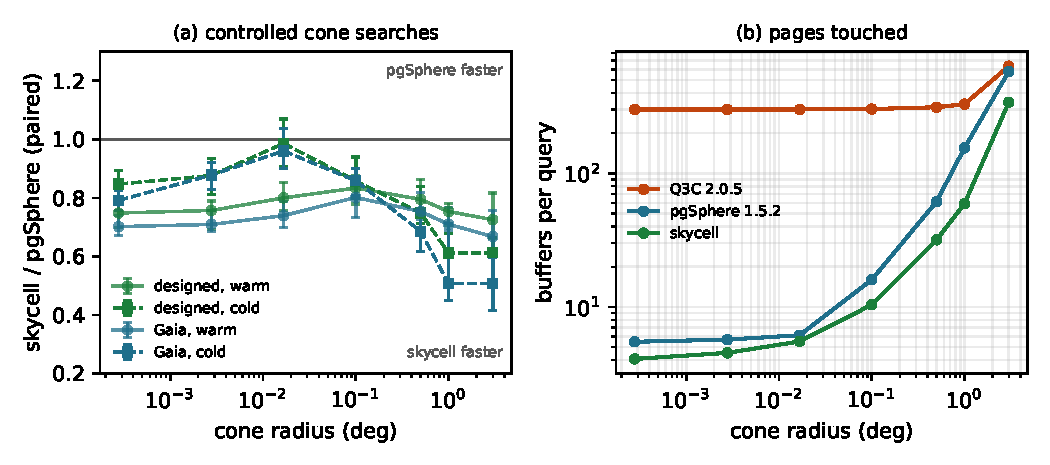
\includegraphics[width=\columnwidth]{fig_benchmark.pdf}
  \caption{\emph{(a)} Paired ratio of \texttt{skycell} to pgSphere against cone radius,
    95\% bootstrap intervals, synthetic catalogues, warm and cold; below the line
    \texttt{skycell} is faster. \emph{(b)} Buffer pages touched per query (mean,
    designed catalogue).}
  \label{fig:benchmark}
\end{figure}

Cone searches are the most common archive query and pgSphere's strength.
Table~\ref{tab:cones} and Fig.~\ref{fig:benchmark} show that, with a warm cache,
\texttt{skycell} is faster than pgSphere at every radius on all three catalogues: by
17--33\% on the two synthetic ones and by 4--31\% on real positions. At 1\arcsec\ it
spends slightly longer planning (0.036\,ms against 0.029) but executes faster (0.022\,ms
against 0.040), reading 4.1 pages to pgSphere's 5.5. Cold, it
is faster or level everywhere, and the margin grows with radius to a factor 1.6--2.1 at
1\degr\ and 3\degr, because it touches about a third of pgSphere's pages there (59
against 155 on the designed catalogue, 85 against 282 on the Gaia one). On real
positions the cold gain is a factor 1.5--2.1 from 6\arcmin\ up; below that a first query
reads only two or three pages and the two methods are about level. These cold numbers
come from fast flash storage, where a saved page is worth about 0.1\,ms; on a slower disk
each saved page counts for more.

Against Q3C, \texttt{skycell} takes 0.02--0.58 of the time. This mostly reflects Q3C
2.0.5's implementation rather than its design: \texttt{q3c\_radial\_query} expands every
call into about 100 bitmap index scans regardless of radius, and spends about 2.7\,ms
planning them. Q3C's cross-match, which does not have this overhead, is the fairer
comparison (\Sect~\ref{sec:xmatch}).

\begin{table*}
  \caption{Cone searches: paired ratio of \texttt{skycell} to pgSphere with its 95\%
    bootstrap interval. Below 1, \texttt{skycell} is faster. \textbf{Bold}: interval
    excludes 1. $n$: distinct queries at that radius. Real catalogue: its own centres at
    the same radii and counts; cold there uses one table per method and fresh centres,
    so neither method warms the other's pages.}
  \label{tab:cones}
  \centering
  \footnotesize
  \setlength{\tabcolsep}{4pt}
  \begin{tabular}{l r cc cc cc}
    \hline\hline
    & & \multicolumn{2}{c}{designed catalogue} & \multicolumn{2}{c}{Gaia catalogue (resampled)} & \multicolumn{2}{c}{real Gaia DR3 positions} \\
    \cline{3-4}\cline{5-6}\cline{7-8}
    radius & $n$ & warm & cold & warm & cold & warm & cold \\
    \hline
    1\arcsec  & 400 & \textbf{0.75} [0.70, 0.79] & \textbf{0.85} [0.80, 0.89] & \textbf{0.70} [0.67, 0.74] & \textbf{0.79} [0.76, 0.83] & \textbf{0.83} [0.81, 0.84] & \textbf{0.87} [0.82, 0.94] \\
    10\arcsec & 400 & \textbf{0.76} [0.69, 0.79] & \textbf{0.88} [0.81, 0.94] & \textbf{0.71} [0.68, 0.76] & \textbf{0.88} [0.83, 0.92] & \textbf{0.85} [0.82, 0.86] & 1.01 [0.94, 1.09] \\
    1\arcmin  & 300 & \textbf{0.80} [0.76, 0.85] & 0.99 [0.91, 1.07] & \textbf{0.74} [0.70, 0.79] & 0.96 [0.90, 1.04] & \textbf{0.90} [0.87, 0.92] & 0.98 [0.90, 1.04] \\
    6\arcmin  & 200 & \textbf{0.83} [0.78, 0.88] & \textbf{0.86} [0.80, 0.94] & \textbf{0.80} [0.74, 0.86] & \textbf{0.86} [0.81, 0.90] & \textbf{0.96} [0.93, 0.99] & \textbf{0.61} [0.55, 0.65] \\
    30\arcmin & 100 & \textbf{0.79} [0.75, 0.86] & \textbf{0.75} [0.71, 0.84] & \textbf{0.75} [0.73, 0.82] & \textbf{0.69} [0.62, 0.76] & \textbf{0.81} [0.78, 0.86] & \textbf{0.67} [0.60, 0.72] \\
    1\degr    &  40 & \textbf{0.75} [0.71, 0.78] & \textbf{0.61} [0.52, 0.68] & \textbf{0.71} [0.69, 0.77] & \textbf{0.51} [0.45, 0.72] & \textbf{0.80} [0.75, 0.88] & \textbf{0.53} [0.44, 0.66] \\
    3\degr    &  16 & \textbf{0.73} [0.66, 0.82] & \textbf{0.61} [0.50, 0.66] & \textbf{0.67} [0.63, 0.76] & \textbf{0.51} [0.41, 0.60] & \textbf{0.69} [0.64, 0.75] & \textbf{0.48} [0.43, 0.54] \\
    \hline
  \end{tabular}
\end{table*}

\subsection{Catalogue size, index size and build time}
\label{sec:scale}
\label{sec:scale-memory}

Ten million rows is 0.55\% of Gaia DR3, so the tests were repeated at 50 million rows.
At that size pgSphere's index (3439\,MB) no longer fits in the 2\,GB buffer pool, while
\texttt{skycell}'s (1071\,MB) still does (Table~\ref{tab:scale}). With a warm cache
\texttt{skycell} stays 14--31\% faster at every radius. Cold, its lead grows with
catalogue size from 30\arcmin\ up, to a factor 1.9 at 30\arcmin, 2.7 at 1\degr\ and 2.4
at 3\degr, as the gap in pages read widens (188 against pgSphere's 642 at 1\degr). Its
row estimates, which the planner uses to choose join strategies, stay within a factor
1.3 of the truth, while pgSphere's are off by up to a factor 8.7 and Q3C's by up to 2.4.

\begin{table}
  \caption{Paired ratio of \texttt{skycell} to pgSphere on the Gaia density field at two
    catalogue sizes. \textbf{Bold}: interval excludes 1.}
  \label{tab:scale}
  \centering
  \footnotesize
  \begin{tabular}{@{}l cc cc@{}}
    \hline\hline
    & \multicolumn{2}{c}{warm} & \multicolumn{2}{c}{cold} \\
    \cline{2-3}\cline{4-5}
    radius & $10^7$ & $5{\times}10^7$ & $10^7$ & $5{\times}10^7$ \\
    \hline
    1\arcsec  & \textbf{0.70} & \textbf{0.78} & \textbf{0.79} & \textbf{0.82} \\
    10\arcsec & \textbf{0.71} & \textbf{0.78} & \textbf{0.88} & \textbf{0.86} \\
    1\arcmin  & \textbf{0.74} & \textbf{0.86} & 0.96          & 0.98          \\
    6\arcmin  & \textbf{0.80} & \textbf{0.86} & \textbf{0.86} & \textbf{0.81} \\
    30\arcmin & \textbf{0.75} & \textbf{0.75} & \textbf{0.69} & \textbf{0.53} \\
    1\degr    & \textbf{0.71} & \textbf{0.69} & \textbf{0.51} & \textbf{0.37} \\
    3\degr    & \textbf{0.67} & \textbf{0.73} & \textbf{0.51} & \textbf{0.42} \\
    \hline
  \end{tabular}
\end{table}

Index size and build time decide how much memory a server needs and how long a new
catalogue release takes to index. The cost per row is flat between $10^7$ and $5\times10^7$ rows, so it can be
extrapolated to Gaia DR3's $1.81\times10^9$ sources (Table~\ref{tab:gaia}). The
relevant comparison is between deployments: an archive that serves both cone searches
and cross-matches today typically runs pgSphere plus Q3C, whose \texttt{q3c\_join} is
2.4--2.6 times faster than pgSphere at cross-matching (\Sect~\ref{sec:xmatch}).
\texttt{skycell} serves both from one index. At DR3 scale that is 38\,GiB against
160\,GiB, the difference between a 64\,GiB and a 256\,GiB server, and an index build of
10 minutes against 4.1 hours. The smaller index also helps when memory is short: in a
3\,GiB container with 768\,MB of shared buffers and a 22\,GB, 20.5-million-row
ObsCore-shaped table, where pgSphere's index is 1.5 times the buffer pool and
\texttt{skycell}'s 0.57 times, \texttt{skycell} answered a stream of 2\degr\ cones
across the sky 4.2--4.8 times faster.

\begin{table}
  \caption{Index size and build time at $10^7$ rows, and extrapolated linearly from the
    $5\times10^7$ measurement to Gaia DR3 ($1.81\times10^9$ sources). Last column: the
    smallest conventional server memory holding the index with room for the table.}
  \label{tab:gaia}
  \centering
  \footnotesize
  \begin{tabular}{@{}l rr rrr@{}}
    \hline\hline
    & \multicolumn{2}{c}{$10^7$ rows} & \multicolumn{3}{c}{at Gaia DR3 scale} \\
    \cline{2-3}\cline{4-6}
    index & MB & build (s) & GiB & build & mem GiB \\
    \hline
    Q3C              & 214 &  5.6 & 38 & 15\,min & 64 \\
    pgSphere         & 685 & 68.6 & 122 & 3.9\,h & 192 \\
    skycell          & 214 &  6.0 & \textbf{38} & 10\,min & 64 \\
    \hline
    pgSphere $+$ Q3C & --- & --- & 160 & 4.1\,h & 256 \\
    \hline
  \end{tabular}
\end{table}

\subsection{Cross-matching and polygons}
\label{sec:xmatch}
\label{sec:otherops}

Cross-matching an uploaded target list is Q3C's speciality, so it is the main test of
the B-tree design against Q3C's. On real Gaia DR3 positions, at the radii cross-matching
uses (1--1.5\arcsec\ for optical, up to 5\arcsec\ for radio) and with uploads of
$10^3$--$10^5$ targets, clustered or uniform (Table~\ref{tab:xmreal}), \texttt{skycell}
takes 0.79 of \texttt{q3c\_join}'s time and 0.32 of pgSphere's overall, and is faster
than both in all 24 test cells. On the resampled catalogue, with 200\,000 targets at
1\arcsec\ and 10\arcsec, it takes 0.67--0.75 of \texttt{q3c\_join}'s time and
0.26--0.31 of pgSphere's, with identical results. The gain comes from covering each
target's cone with only the ranges it needs, 1.2 on average at 1\arcsec\ (4.3 pages per
target). The join can be written with \texttt{skycell\_cone}, \texttt{skycell\_join} or
ADQL's \texttt{point <@ circle}; all three produce the same plan.

Convex polygons of 0.05\degr--2\degr\ take a median 0.28\,ms against pgSphere's 0.77 and
Q3C's 1.86, a factor 2.7--4.4 on both synthetic catalogues; pgSphere's slowest queries
are far above its median when a polygon's bounding volume fits it poorly.

\begin{table}
  \caption{Cross-matching on real Gaia DR3 positions ($10^7$ rows): geometric mean over
    three upload sizes ($10^3$--$10^5$) and two target distributions of the per-cell
    ratio of median times, method order random per cell. \emph{Cone}: the join written
    with \texttt{skycell\_cone}; \emph{join}: with \texttt{skycell\_join}, Q3C's
    spelling. Below 1, \texttt{skycell} is faster; \textbf{bold}: faster in every cell.}
  \label{tab:xmreal}
  \centering
  \footnotesize
  \begin{tabular}{l rr r}
    \hline\hline
    & \multicolumn{2}{c}{vs \texttt{q3c\_join}} & vs pgSphere \\
    \cline{2-3}\cline{4-4}
    radius & cone & join & join \\
    \hline
    $0.5\arcsec$ & \textbf{0.81} & \textbf{0.77} & \textbf{0.30} \\
    $1\arcsec$   & \textbf{0.77} & \textbf{0.76} & \textbf{0.30} \\
    $1.5\arcsec$ & \textbf{0.77} & \textbf{0.78} & \textbf{0.34} \\
    $5\arcsec$   & \textbf{0.84} & \textbf{0.83} & \textbf{0.35} \\
    \hline
    all          & \textbf{0.80} & \textbf{0.79} & \textbf{0.32} \\
    \hline
  \end{tabular}
\end{table}

\subsection{An observation table}
\label{sec:tap}

Observation tables cluster around field centres and are often ordered by collection,
not position. An ObsCore-shaped table, with observations in groups of 128 sharing a field centre, was
built at three sizes and asked the same 30 queries at each (Table~\ref{tab:crossover}).
\texttt{skycell}'s lead grows with table size: at $10^7$ rows it is level on the
0.15\degr\ cone and faster in every other class, by 25\% on the 2\degr\ cone, where
pgSphere reads 939 pages to its 591. pgSphere wins only the small cone on the smallest
table, where its bitmap scan already reads exactly the pages needed. On tables that
small the index choice matters little anyway: inside a TAP 1.1 service \citep{egernia} on
a 500\,000-row ObsCore table, the two indexes gave the same throughput at 1--32
concurrent clients, because the service's own code costs about 10\,ms per request
against a fraction of a millisecond in the database.

\begin{table}
  \caption{ObsCore-shaped table at three sizes: total query time of \texttt{skycell} as
    the ratio to pgSphere (pgS.), 30 stored centres, two complete randomized runs
    pooled; median buffer pages at $10^7$ rows. Q05: 0.15\degr\ cone; Q06: 2\degr;
    Q07: 0.5\degr\ with calibration and time cuts; Q12: an empty 0.7\arcsec\ cone.}
  \label{tab:crossover}
  \centering
  \footnotesize
  \setlength{\tabcolsep}{3pt}
  \begin{tabular}{l rrr rr}
    \hline\hline
    & \multicolumn{3}{c}{\texttt{skycell} / pgS.} & \multicolumn{2}{c}{buffers, $10^7$} \\
    \cline{2-4}\cline{5-6}
    rows ($10^6$) & 0.5 & 2 & 10 & pgS. & skycell \\
    \hline
    Q05 & 1.14 & 1.07 & 0.97 &  32 &  32 \\
    Q06 & 0.92 & 0.93 & 0.75 & 939 & 591 \\
    Q07 & 0.94 & 0.99 & 0.80 & 113 &  89 \\
    Q12 & 0.71 & 0.68 & 0.47 &   7 &   3 \\
    \hline
  \end{tabular}
\end{table}

\subsection{How reliable is the density estimate?}
\label{sec:estimator}
\label{sec:ablation}

Table~\ref{tab:estimator} compares the density estimate of Eq.~(\ref{eq:rho}) with the
density counted from the real-position catalogue. It is within 5\% in Baade's Window and a
factor 1.3 at the Galactic pole, but low by a factor 10--50 in globular cluster cores and
high by 3.7 at the Galactic centre: the histogram resolves a cluster while the query
sits inside it, but averages it away once the query is larger. The effect on queries is
much smaller than the error. Since $s_\star\propto\rho^{-1/2}$, an error of ten in the
density changes the cell size by about three, and the cost curve is flat over much of
that range. In cluster cores the covering chosen is within 1.05--1.53 of the best fixed
cell size, and within 0.98--1.31 elsewhere, whereas a badly chosen fixed size is
243--830 times worse.

\begin{table}
  \caption{The density estimate $\hat\rho$ against the true density $\rho$ on real Gaia
    DR3 positions, radii 0.01\degr--1\degr: median ratio over radii, then over ten
    \texttt{ANALYZE} samples; \emph{samples}: spread of that median across them;
    \emph{range}: over all radii and samples.}
  \label{tab:estimator}
  \centering
  \footnotesize
  \begin{tabular}{l rrr}
    \hline\hline
    field & $\hat\rho/\rho$ & samples & range \\
    \hline
    $\omega$~Cen           & \textbf{0.08} & 0.06--0.09 & 0.05--0.54 \\
    47~Tuc                 & \textbf{0.02} & 0.01--0.11 & 0.00--0.94 \\
    LMC                    & 0.80 & 0.46--0.92 & 0.22--1.26 \\
    Baade's Window         & 0.96 & 0.92--0.98 & 0.45--1.19 \\
    Galactic pole          & 1.27 & 1.18--1.49 & 0.48--1.69 \\
    Galactic centre        & \textbf{3.71} & 3.41--3.80 & 1.95--5.20 \\
    \hline
  \end{tabular}
\end{table}

\subsection{Stored regions}
\label{sec:tests-regions}

The GiST index was tested on the real 50\,000-row \texttt{fpr} footprint catalogue
against pgSphere's native GiST index. With the default box key, \texttt{skycell} is
faster for all four region operators (Table~\ref{tab:gistregion}), from 6--8 times
faster for overlap to 7--25\% faster for finding the footprints that contain a
position. On footprints of a single size it reads 10--25\% fewer buffer pages in
10--20\% less time, and on a column mixing circles and polygons the margin widens,
because pgSphere has to search one index per region type. For the point-in-footprint
query, storing footprints as MOC cells in a B-tree answered 200\,474 point-in-region
pairs in 0.76\,s against pgSphere's 0.97\,s.

\begin{table}
  \caption{Region operators on the 50\,000-row \texttt{fpr} catalogue, 500 probes per
    operator: time of the box-key GiST index as the ratio to pgSphere's native GiST.
    Below 1, \texttt{skycell} is faster.}
  \label{tab:gistregion}
  \centering
  \footnotesize
  \begin{tabular}{l r}
    \hline\hline
    operator & box key / pgSphere \\
    \hline
    \texttt{\&\&} (overlap) & \textbf{0.12--0.17} \\
    \texttt{@>}(region,point) & \textbf{0.75--0.93} \\
    \texttt{@>}(region,region) & \textbf{0.55--0.70} \\
    \texttt{<@}(region,region) & \textbf{0.26--0.27} \\
    \hline
  \end{tabular}
\end{table}

\section{Conclusions}
\label{sec:conclusions}

\texttt{skycell} keeps Q3C's compact integer key and B-tree, chooses each covering's
resolution from local source density and the cost of an index range, and adds a GiST
index for stored regions. Compared directly with the two extensions archives use today,
it is faster than each at its own speciality: cone searches are faster than with
pgSphere at every radius from 1\arcsec\ to 3\degr\ with a warm cache (by 17--33\% on
synthetic catalogues and 4--31\% on real Gaia DR3 positions), faster or level when cold,
and further ahead as the catalogue grows; cross-matches are 20--33\% faster than
\texttt{q3c\_join} and about three times faster than pgSphere. Convex polygons run
2.7--4.4 times faster than with pgSphere, and the region index is faster than
pgSphere's on every operator tested.

For an archive the operational gains may matter as much: one index, a third the size of
pgSphere's and built 11--23 times faster, replaces the pgSphere-plus-Q3C pair, with
nothing to tune. Adoption needs only an expression index on existing \texttt{ra} and
\texttt{dec} columns, and queries keep ADQL's own names. This makes \texttt{skycell} a
strong candidate for the positional layer of a PostgreSQL archive or TAP service.

The gains are smallest on small tables, where planning a covering is a larger share of
each query and a small cone on $5\times10^5$ rows can still favour pgSphere; there, as
inside a TAP service dominated by its own code, an existing index is good enough.


\section*{CRediT authorship contribution statement}

\textbf{Jes\'us Salgado:} Conceptualization, Methodology, Software, Formal analysis,
Writing -- original draft. \textbf{Michele Delli Veneri:} Validation, Investigation,
Writing -- review \& editing.

\section*{Declaration of competing interest}

The authors declare that they have no known competing financial interests or personal
relationships that could have appeared to influence the work reported in this paper.

\section*{Declaration of generative AI and AI-assisted technologies in the writing process}

During the preparation of this work the authors used Claude Code (Anthropic) in order to
develop the software, the benchmark harness and the analysis, and to draft the
manuscript. After using this tool, the authors reviewed and edited the content as needed
and take full responsibility for the content of the published article. The geometric
predicates and coverings are checked by the brute-force suites of
Section~\ref{sec:validation} against independent computations over millions of
adversarially placed points rather than expected outputs, and every indexed answer in the
regression suites must equal a sequential scan with the exact predicate.

\section*{Data availability}

The extension, its test suites, the benchmark harness and the raw results of every
measurement quoted here are available at
\url{https://github.com/jesusjuansalgado/skycell} under the MIT licence, together with
the history of the measurements that led to the current defaults. All corpora but the
real one are generated from seeds; the real one is drawn from the Gaia archive by a
recorded query.

\section*{Acknowledgements}

This work has made use of data from the European Space Agency (ESA) mission \emph{Gaia}
(\url{https://www.cosmos.esa.int/gaia}), processed by the \emph{Gaia} Data Processing and
Analysis Consortium (DPAC, \url{https://www.cosmos.esa.int/web/gaia/dpac/consortium}).
Funding for the DPAC has been provided by national institutions, in particular the
institutions participating in the \emph{Gaia} Multilateral Agreement.

\section*{Funding}

This research did not receive any specific grant from funding agencies in the public,
commercial, or not-for-profit sectors.

\begin{thebibliography}{}

\bibitem[Chilingarian et al.(2004)]{pgsphere}
Chilingarian, I., Bartunov, O., Richter, J., \& Sigaev, T. 2004,
  in ASP Conf. Ser. 314, Astronomical Data Analysis Software and Systems XIII,
  ed. F. Ochsenbein, M. G. Allen, \& D. Egret (San Francisco: ASP), 225

\bibitem[Delli Veneri \& Salgado(2026)]{egernia}
Delli Veneri, M., \& Salgado, J. 2026, egernia: an IVOA TAP 1.1 server for the SKA
  Observatory, Zenodo, doi:10.5281/zenodo.22845690

\bibitem[Demleitner et al.(2014)]{dachs}
Demleitner, M., Neves, M. C., Rothmaier, F., \& Wambsganss, J. 2014,
  Astron. Comput., 7--8, 27

\bibitem[Dowler et al.(2019)]{tap}
Dowler, P., Rixon, G., Tody, D., \& Demleitner, M. 2019,
  IVOA Recommendation: Table Access Protocol Version 1.1

\bibitem[ESA(1997)]{hipparcos}
ESA 1997, The Hipparcos and Tycho Catalogues, ESA SP-1200

\bibitem[Fernique et al.(2014)]{moc}
Fernique, P., Boch, T., Donaldson, T., et al. 2014,
  IVOA Recommendation: MOC -- HEALPix Multi-Order Coverage map Version 1.0

\bibitem[Gaia Collaboration(2016)]{gaia}
Gaia Collaboration, Prusti, T., de Bruijne, J. H. J., et al. 2016, A\&A, 595, A1

\bibitem[G\'orski et al.(2005)]{healpix}
G\'orski, K. M., Hivon, E., Banday, A. J., et al. 2005, ApJ, 622, 759

\bibitem[Gray et al.(2006)]{zones}
Gray, J., Nieto-Santisteban, M. A., \& Szalay, A. S. 2006,
  The Zones Algorithm for Finding Points-Near-a-Point or Cross-Matching Spatial
  Datasets, Microsoft Research Technical Report MSR-TR-2006-52

\bibitem[Koposov \& Bartunov(2006)]{q3c}
Koposov, S., \& Bartunov, O. 2006, in ASP Conf. Ser. 351, Astronomical Data
  Analysis Software and Systems XV, ed. C. Gabriel, C. Arviset, D. Ponz, \&
  S. Enrique (San Francisco: ASP), 735

\bibitem[Kunszt et al.(2001)]{htm}
Kunszt, P. Z., Szalay, A. S., \& Thakar, A. R. 2001, in Mining the Sky,
  ed. A. J. Banday, S. Zaroubi, \& M. Bartelmann (Berlin: Springer), 631

\bibitem[Moon et al.(2001)]{hilbert}
Moon, B., Jagadish, H. V., Faloutsos, C., \& Saltz, J. H. 2001,
  IEEE Trans. Knowl. Data Eng., 13, 124

\bibitem[Ortiz et al.(2008)]{adql}
Ortiz, I., Lusted, J., Dowler, P., et al. 2008,
  IVOA Recommendation: Astronomical Data Query Language Version 2.0

\bibitem[Rots(2007)]{stc}
Rots, A. H. 2007, IVOA Recommendation: Space-Time Coordinate Metadata for
  the Virtual Observatory Version 1.33

\bibitem[Salgado et al.(2017)]{gaiaarchive1}
Salgado, J., Gonz\'alez-N\'u\~nez, J., Guti\'errez-S\'anchez, R., et al. 2017,
  Astron. Comput., 21, 22

\bibitem[Salgado et al.(2020)]{gaiaarchive2}
Salgado, J., et al. 2020, in ASP Conf. Ser. 522, Astronomical Data Analysis
  Software and Systems XXVII, ed. P. Ballester, J. Ibsen, M. Solar, \&
  K. Shortridge (San Francisco: ASP), 307

\end{thebibliography}


\end{document}
